\documentclass[windows,csize4]{BHCexam}
%\documentclass[windows,csize4,answers]{BHCexam}

\usepackage{multicol} % 分栏
\usepackage{polynom} % 多项式除法
\pagestyle{fancy}
\fancyfoot[C]{\kaishu \small 第 \thepage 页 共 \pageref{lastpage} 页}
%\fancyhead[L]{\includegraphics[width=2cm]{qrcode.png}}
\title{声音}
%\subtitle{数学文科试卷}
%\notice{满分150分, 120分钟完成, \\	允许使用计算器,答案一律写在答题纸上.}
%\author{Gavin Chen}
%\date{\today}
\usepackage{enumerate} % 编号
\usepackage{cases}
\usepackage{subfigure}
\usepackage{graphicx}

\begin{document}

\maketitle

\begin{groups}
    \group{声音的产生与传播}{}
    声音是如何产生的?
    \begin{itemize}
        \item 由物体振动产生。振动停止,声音停止。
        \item 声源:正在发声的物体。
        \item 固体、液体、气体都可以振动产生声音。
    \end{itemize}

    声音是如何传播的?
    \begin{itemize}
        \item 声音传播需要介质。例子:把闹钟放在密封空间抽空气,声音越来越轻。(真空不能传递声音)
        \item 声音在不同介质中的传播速度,一般来说,传播速度固体>液体>气体。
        \item 声音以波的形式传播,称之为声波。
    \end{itemize}

    人耳听到声音,通常是由空气传播,然后进入耳道。但是也可以用骨传导耳机。(据说贝多芬耳朵聋了之后就采用类似方法作曲)

    想一想,如果声源在移动,会不会影响声音传播的速度?比如救护车疾驶而过,这个时候声音通过空气传播,那么救护车的速度会不会影响它发出的警报声在空气中的传播速度呢?

    \group{声音的特征}{}

    人耳感觉到的声音的强弱程度叫做响度。想一想,下图中两个声波,那个更响?
    图 \ref{fig:fig_2_1}声波的形状和响度
    \begin{figure}[htb]
        \centering
        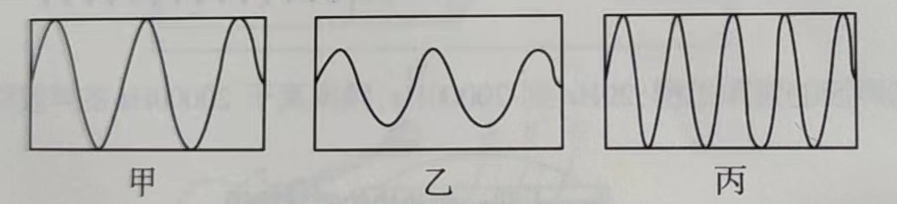
\includegraphics [scale=0.5,trim=0 0 0 0]{./image/fig_2_1.PNG}
        \caption{声波的形状和响度}
        \label{fig:fig_2_1}
    \end{figure}

    影响响度的因素
    \begin{itemize}
        \item 响度和振幅有关,振幅越大,响度越大。
        \item 响度和接收者离开声源的距离有关,距离越近,响度越大。
        \item 利用喇叭,可以是声波的传播方向更加集中,可以在不改变距离和声源振幅的情况下增加响度及传播更远的距离。
    \end{itemize}

    音调:声音的高低。有时也叫做音高。比如常说的男高音,女中音就是指的音调。

    \begin{itemize}
        \item 音调和发声体振动的快慢(即频率)有关。
        \item 频率:物体每秒钟振动的次数,单位:次/秒。即赫兹(Hz)
        \item 频率的物理意义:反映物体振动快慢。
        \item 频率低,音调低
    \end{itemize}

    回到图 \ref{fig:fig_2_1}中,甲和丙什么一样,什么不一样?
    回到刚才救护车的例子,声音传播的速度没变,但是什么变了?

    图 \ref{fig:fig_2_2}声音的频率,数一下下面两者的频率分别是多少?
    \begin{figure}[htb]
        \centering
        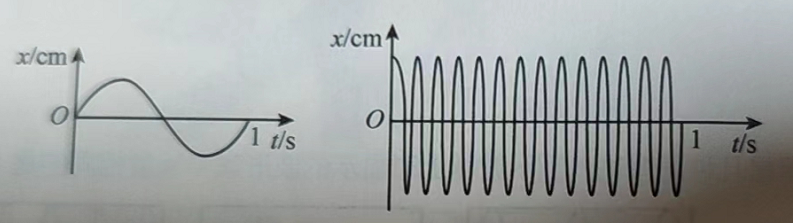
\includegraphics [scale=0.3,trim=0 0 0 0]{./image/fig_2_2.PNG}
        \caption{声音的频率}
        \label{fig:fig_2_2}
    \end{figure}

    小知识,人耳的听觉范围$20Hz~20000Hz$,常见动物的听力和发声频率,见图 \ref{fig:fig_2_3}.
    \begin{figure}[htb]
        \centering
        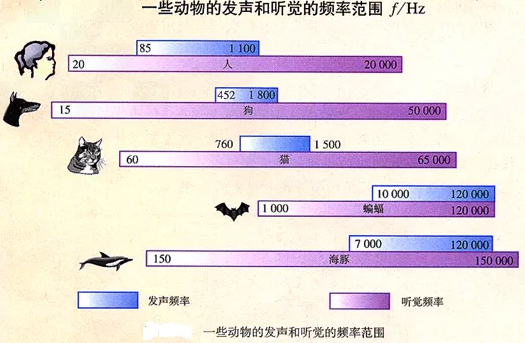
\includegraphics [scale=0.75,trim=0 0 0 0]{./image/fig_2_3.PNG}
        \caption{声音的频率}
        \label{fig:fig_2_3}
    \end{figure}

    小知识,对弦乐类乐器,其音调和弦的粗细、长短、松紧程度有关系。弦越短,越细,越紧,那么音调就越高;对管乐类乐器,一般其空气柱长度越短,音调越高。

    音色,声音的特色,是我们分辨各种声音的依据。比如钢琴和小提琴的音色不一样。
    \begin{itemize}
        \item 发声体本身的材料、结构是影响音色的主要因素。
        \item 发声体发出的声音一般不是单一的频率,而是各个频率声波的组合。频率的组合情况不同,音色就不同。
    \end{itemize}

    \begin{figure}[htb]
        \centering
        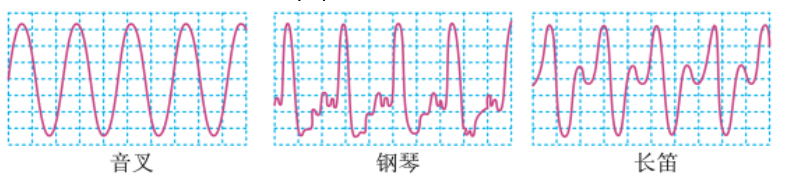
\includegraphics [scale=0.6,trim=0 0 0 0]{./image/fig_2_4.PNG}
        \caption{音叉,钢琴和长笛的音色}
        \label{fig:fig_2_4}
    \end{figure}
    想一想,图\ref{fig:fig_2_4}中,响度一样嘛?音调一样嘛?音色一样嘛?



    噪音和乐音
    \begin{itemize}
        \item 环境学中,把对人们休息,工作,学习产生干扰的声音叫噪音。
        \item 物理学中,把声体无规则振动发出的声音叫噪音。小知识:宇宙背景辐射。
    \end{itemize}
    噪声的单位:分贝(dB)。 0dB是人们刚能听到的最微弱的声音。
    \begin{figure}[htb]
        \centering
        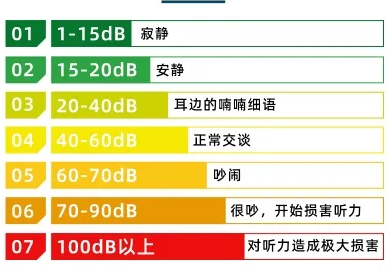
\includegraphics [scale=0.75,trim=0 0 0 0]{./image/fig_2_5.PNG}
        \caption{常见声音的大小}
        \label{fig:fig_2_5}
    \end{figure}
    想一想,如何减弱噪音?
    \begin{itemize}
        \item 声源处:加消音器,禁止鸣笛
        \item 传播过程中:隔音墙,绿化
        \item 人耳处:噪音耳塞
    \end{itemize}
    乐音:悠扬悦耳,令人心旷神怡的声音。

    \group{如何利用声音}{}
    声音技能传递信息,也能传递能量。
    \begin{itemize}
        \item 声音传递信息:超声检查,回声定位
        \item 声音传播能量:超声碎石,超声清洁玻璃
    \end{itemize}

    \group{例题}{}

    \begin{questions}[]
        \question[5]无风的天气,即将进站的列车发出一次鸣号声,持续时间为$5.1s$,若列车的速度为$20m/s$,空气中的声速为$340m/s$,则站台上的人听到鸣号声持续的时间为
        鸣笛声持续时间为多少?站台附近一辆以速度$20m/s$同向行驶的车上乘客听到的时间为多少?
        \begin{solution}{0.5cm}
            \methodonly 列车和声音传播同向,相当于“追”着声音前进,声波被压缩。(弹簧模型)\\
            $t'=\frac{L_{A'B}}{v_{voice}}=\frac{(v_{voice}-v_{train})t}{v_{voice}}=\frac{(340m/s-20m/s)\times 5.1s}{340m/s}=4.8s$

            对于同向行驶的列车上的人而言,辆车相对静止,故仍然是$5.1s$;或者理解成“弹簧”相对于乘客的速度是$(340-20)m/s$。\\
            想一想,为什么要强调是无风的天气?如果站台上有一辆相向行驶的列车,又是怎样一种情况呢?
        \end{solution}
        \vspace{3.5cm}

        \question[5]火车以$20m/s$的速度沿某一段直线轨道驶向道口,为了提醒看守口的工作人员,
        司机在距道口$940m$处开始鸣响汽笛,每次笛声持续$1s$,停$5s$,然后再次拉响汽笛。当道口工作人员听到第三次笛声结束时,火车距道口距离多少米?
        道口工作人员听到火车司机前后两次拉响汽笛的时间间隔为多少秒?(已知声波在空气中传播的速度为340m/s)
        \begin{solution}{0.5cm}
            \methodonly 三声汽笛共$13s$,这期间火车开了$260m$,离开工作人员$680m$。但是声音传播还需要时间,以结束时刻为准,还需$\frac{680m}{340m/s}=2s$才
            传到道口,火车还能行驶$40m$。故第三声结束时距离道口$640m$。\\
            如果第一小题都以弹簧模型考虑,需要计算两个部分,1. 声音开始时刻传到道口的时间;道口从开始听到知道最后一声结束的持续时间。两部分相加为$15s$。不如直接从
            时刻计算方便。\\
            第二小问,时间间隔都已听到汽笛的起始点为准。
            $t'=\frac{L_{A'B}}{v_{voice}}=\frac{(v_{voice}-v_{train})t}{v_{voice}}=\frac{(340m/s-20m/s)\times 5s}{340m/s}=5.65s$
        \end{solution}
        \vspace{3.5cm}

        \question[5] 一辆客车在某高速公路上行驶,在经过某直线路段时,司机驾车做匀速直线运动。
        司机发现其将要通过正前方高山悬崖下的隧道,于是鸣笛,$5s$后听到回声,听到回声后又行驶了$10s$后,
        司机第二次鸣笛,$3s$后听到回声。请根据以上数据帮助司机计算一下客车的速度,看客车是否超速行驶,
        以便提醒司机安全行驶,已知此高速公路的最高限速为$120km/h$。
        \begin{figure}[htb]
            \centering
            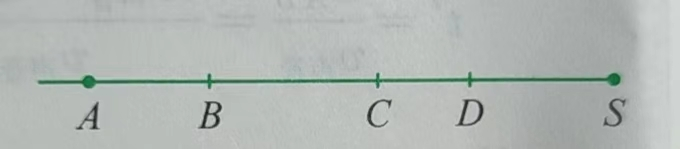
\includegraphics [scale=0.3,trim=0 0 0 0]{./image/fig_2_6.jpg}
            \caption{示意图}
            \label{fig:fig_2_6}
        \end{figure}
        \begin{solution}{0.5cm}
            \methodonly
            由题意$AS+BS=v_{voice}\cdot t_{1}$,
            同时$AB=v_{car}\cdot t_1$,所以$AS=\frac{1}{2}\times (v_{voice}+v_{car})\cdot t_1$。
            同理 $CS=\frac{1}{2}\times (v_{voice}+v_{car})\cdot t_2$ \\
            又$AC=AS-CS=v_{car}\cdot t_3$。
            已知 $t_1=5s,t_2=3s, t_3=15s$,解的$v_{car}=24.3m/s=87.5km/h$
        \end{solution}

        \vspace{3.5cm}

        \question[5] 如图\ref{fig:fig_2_7}所示,停在公路旁的公安巡逻车利用超声波可以监测车速,巡逻车上的测速仪发出并接收超声波脉冲信号,
        根据发出和接收到的信号间的时间差,就能测出车速。在图\ref{fig:fig_2_8}中,$P_1$、$P_2$是测速仪先后发出的超声波信号,$n_1$、$n_2$分别是
        测速仪检测到的$P_1$、$P_2$经反射后的信号。设测速仪匀速扫描,$P_1$与$P_2$之间的时间间隔为$0.9s$,超声波在空气中传播的速度为$340m/s$,
        则被测车的车速为多少?
        \begin{figure}[htb]
            \centering
            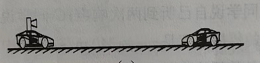
\includegraphics [scale=0.75,trim=0 0 0 0]{./image/fig_2_7.PNG}
            \caption{警车测速示意图}
            \label{fig:fig_2_7}
        \end{figure}
        \begin{figure}[htb]
            \centering
            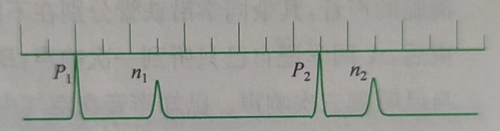
\includegraphics [scale=0.75,trim=0 0 0 0]{./image/fig_2_8.PNG}
            \caption{测速脉冲}
            \label{fig:fig_2_8}
        \end{figure}
        \begin{solution}{0.5cm}
            \methodonly 思考几个问题。1.假设发出型号是车的位置为$m_1$, 车子接受到信号是位置为$m_2$, 信号返回警车时车的位置是$m_3$,这三个位置有什么关系?\\
            显然$m_2$是$m_1$和$m_3$的中点。而中点离开警车的距离是可以通过声速求的。从图中看出,$P_1$、$P_2$间隔$0.9s$,每格$0.1s$,第一次经过$0.15s$信号返回警车,
            第二次经过$0.1s$返回警车,两次离开警车的距离分别是$0.15s\times 340m/s=51m,0.1s\times 340m/s=34m$ 即$0.85s$开了$17m$,即可求得速度。
        \end{solution}

        \question[5] 如图所示,四个相同的玻璃瓶里装水,水面高度不同。用嘴贴着瓶口吹气,如果能分别吹出“do(1)”“re(2)”“mi(3)”“fa(4)”四个音,
        则与这四个音相对应的瓶子的序号分别是什么?
        \begin{figure}[htb]
            \centering
            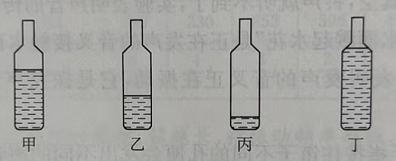
\includegraphics [scale=0.75,trim=0 0 0 0]{./image/fig_2_9.PNG}
            \caption{瓶子中水的多少与音调的关系}
            \label{fig:fig_2_9}
        \end{figure}
        \begin{solution}{0.5cm}
            \methodonly 空气少的音调高
        \end{solution}

        \question[5] 小明同学研究了均匀拉紧的琴弦发音频率与弦长的关系,并记录了实测的数据(如下表所示)。
        请你根据记录表中的有关数据,分析并估算出他有意留出的空格中应该填写的数据(要求写出估算的过程)。
        \begin{figure}[htb]
            \centering
            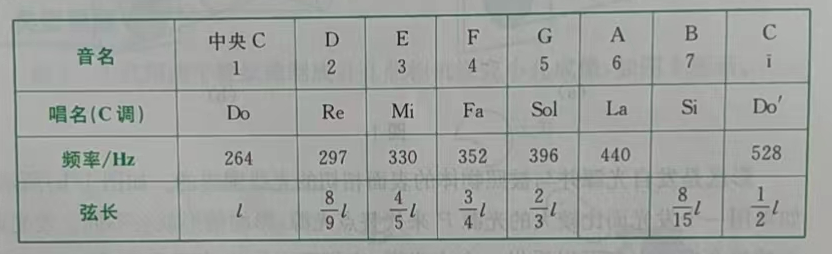
\includegraphics [scale=0.6,trim=0 0 0 0]{./image/fig_2_10.PNG}
            \caption{弦长和频率的关系}
            \label{fig:fig_2_10}
        \end{figure}
        \begin{solution}{0.5cm}
            \methodonly 补充十二平均律和五度相生律相关音乐知识。等比例求解即可
        \end{solution}



    \end{questions}

    \group{作业}{}
    \begin{questions}[]
        \question[5] 潜水艇竖直下沉时,向水底发射出持续时间为$\Delta t_1$的某脉冲声波信号,经一段时间,该潜水艇接收到了反射信号,持续时间为$\Delta t_2$,
        已知声波在水中传播速度为$v_0$,则潜水艇的下沉速度$v_1$是多少?

        \question[5] 假定有前后两次声音传到人的耳朵里,如果这两次声音到达人的耳朵的先后时间间隔大于(或等于)$0.1s$,
        人耳就能够把这两次声音分辨开,也就是说,如果两次声音传到人耳的时间间隔不足 $0.1 s$,人耳就只能听到一次声音。
        某学校8年级课外活动小组为了体验声音在不同介质中的传播速度不同的物理现象,他们请一位同学在输送水的管道(充满水)上敲击一下,
        使铁管发出清脆的声音,其余同学沿铁管分别在不同位置用耳朵贴近铁管听声。实验结束后,A同学说自己只听到一次响声;B同学说自己听到两次响声;
        C同学说自己听到三次响声。已知声音在空气中的传播速度是$v_g=340 m/s$,在水中的传播速度是$v_l=1500 m/s$,在钢铁中的传播速度是$v_s=5100m/s$。
        请你通过计算说明在铁管上某处敲响一次,A、B、C三位同学的位置到达敲击点的距离各在什么范围内?
        \begin{solution}{0.5cm}
            \methodonly 思考一下,如果经过同样的长度,哪两者的时间差小,哪两者的时间差大?这样是不是只需要考虑两种情况即可(哪两种)?
        \end{solution}



    \end{questions}
















\end{groups}




\label{lastpage}
\end{document}